\section{动画变换}\label{sec:动画变换}
\begin{remark}
    本节含有高级内容,第一次阅读时可以跳过。
\end{remark}

\begin{figure}[htbp]
    \centering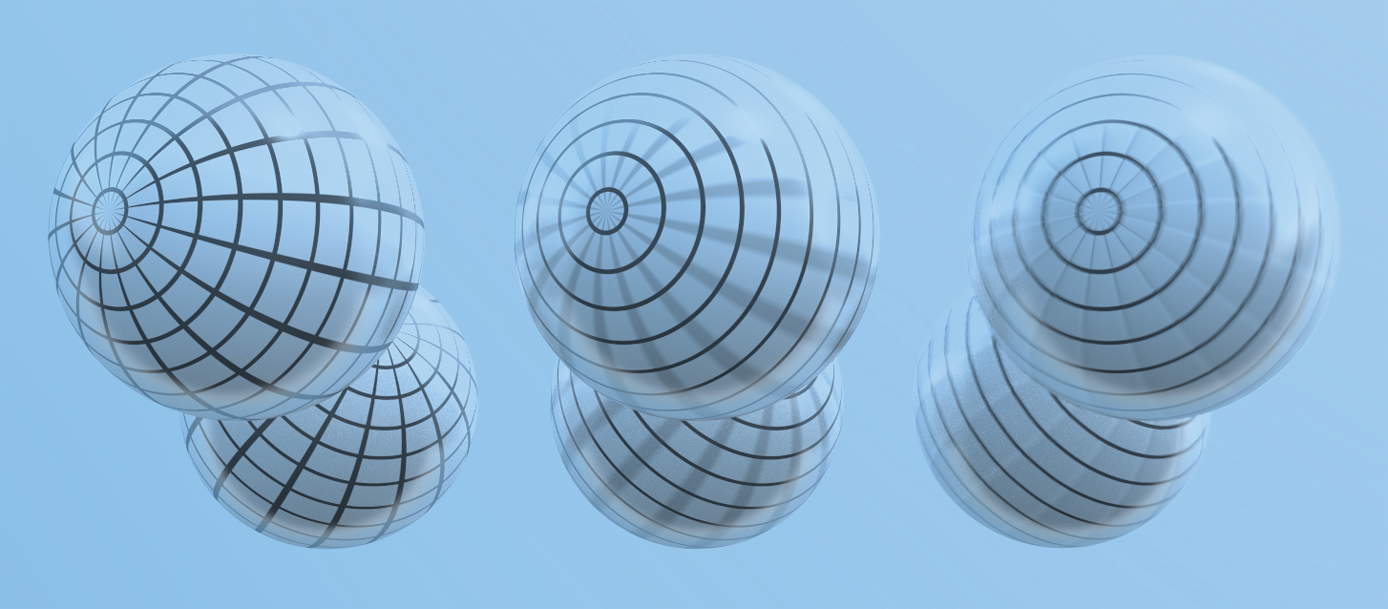
\includegraphics[width=\linewidth]{chap02/spinningspheres.png}
    \caption{转动的球体。用本节实现的变换动画代码以不同速率旋转三个球体并被镜子反射。
        注意球体的反射和球体自身一样模糊。}
    \label{fig:2.15}
\end{figure}

pbrt为场景中的相机和几何图元支持关键帧矩阵动画。
不只是提供单个变换放置场景中的相应物体,
用户还可能提供许多\keyindex{关键帧}{keyframe}{}变换,
每个都与特定时间点关联。
这能让相机移动起来并在仿真相机快门打开时让场景中的物体也移动起来。
\reffig{2.15}展示了三个运用pbrt关键帧矩阵动画的运动球体。

通常,